\documentclass[conference]{IEEEtran}
\usepackage[spanish, activeacute]{babel}
\usepackage[utf8]{inputenc}
\usepackage{amsmath, amssymb}
\usepackage{graphicx}
\usepackage{anysize}
\usepackage{hyperref}
\usepackage{caption}
\usepackage[table]{xcolor}
\usepackage{booktabs}

\usepackage{color}
\newcommand{\todo}{\textcolor{red}{TO DO:}\textcolor{blue}}

\title{ChiVO: estado actual del observatorio virtual chileno}
\author{
\IEEEauthorblockN{
    Jonathan Antognini \IEEEauthorrefmark{1},
    Mauricio Araya     \IEEEauthorrefmark{1},
    Mauricio Solar     \IEEEauthorrefmark{1} \\
}
\IEEEauthorblockA{
    \IEEEauthorrefmark{1} Universidad Técnica Federico Santa María,Valparaiso, Chile}
}

\begin{document}

\maketitle

\begin{abstract}
\end{abstract}

\begin{IEEEkeywords}
\end{IEEEkeywords}

\section{Introducción}

\subsection{Big Data en Astronomía}

En los últimos años, los ámbitos empresarial, científicos y de la administración
han estado haciendo frente a la avalancha de datos con un nuevo concepto que ha
definido como Big Data. Por la simple denominación usada se entiende que se trata
de grandes volúmenes de información que no es sencillo tratar con las herramientas
y procedimientos tradicionales. Encierra esta idea el tratamiento de información
que hizo evolucionar los métodos y recursos habituales para hacerse cargo de grandes
volúmenes de datos (de terabytes a zetabytes). Estos se generan a gran
velocidad y además se añade una posible componente de complejidad y variabilidad en
el formato de esos datos. Las instalaciones astronómicas de última generación
existentes y las que están en construcción, como el Atacama Large
Millimeter/submillimeter Array(ALMA), Large Synoptic Survey Telescope (LSST), y el
Square Kilometer Array (SKA), producirán datos de gran escala que se proyecta que
en el año 2020 generarán más de 60 Petabytes de datos accesibles a los astrónomos.

Todo ello requiere de técnicas y tecnologías específicas para su captura,
almacenamiento, distribución, gestión y análisis de la información.

Big Data no es una tecnología en sí misma, sino más bien un planteamiento de
trabajo para la obtención de valor y beneficios de los grandes volúmenes de
datos que se están generando hoy en día. Se deben contemplar aspectos como:

\begin{itemize}
    \item Cómo capturar, gestionar y explotar
    \item Cómo asegurar, verificar validez y fiabilidad.
    \item Cómo compartir para obtener mejoras y beneficios.
    \item Cómo comunicar para facilitar la toma de decisión y posteriores análisis.
\end{itemize}

\subsection{Observatorios en Chile}

Las privilegiadas condiciones atmosféricas hacen de Chile uno de los lugares más
propicios para la realización de investigaciones científicas en astronomía.

Existen más de una docena de instalaciones astronómicas de gran envergadura a lo
largo de nuestro territorio nacional \cite{observatorios_chile}, como por ejemplo
``Atacama Large Milimeter/submilimeter Array'' (ALMA), ``Very Large Telescope''
(VLT), y en los próximos ``European Extremely Large Telescope'' (E-ELT), con el cual
se estima que el 60\% de la observación astronómica mundial se realice en Chile.
Una de las condiciones que se establecen a nivel país, es que el 10\% del tiempo de
observación pertenece a la comunidad astronómica chilena.
Estos generan datos a gran escala, justificando a nivel país, el desarrollo de una
plataforma astroinformática para su administración y análisis inteligente.

Esto como necesidad no es nuevo, desde el 2002 se pensó en este tipo de problemática
y una forma de abordarlo fue creando el Observatorio Virtual (VO).
El VO es una iniciativa internacional que permite el acceso a archivos astronómicos
y centros de datos a astrónomos y personas comunes a través de Internet.
Con la estandarización de métodos e información es posible estudiar los registros
astronómicos sin requerimientos físicos de instrumentos y locación.

\subsection{¿Por qué es nuevo?}
VO con datos de ALMA.

Resumen de lo importante del paper.

%\subsection{IVOA Standards}


\subsection{ALMA + Cubos + Formatos propios}

\section{Arquitectura de ChiVO}

\subsection{Requerimientos}

Para la creación del ChiVO se identificaron las necesidades actuales de la comunidad
astronómica:

\begin{description}
    \item[Descubrir:] \hfill \\
        Encontrar datos astronómicos de un objeto y/o instrumento sobre una región
        específica del espacio de alta dimensión, en base a parámetros de los ejes
        espaciales, temporales, espectrales, corrimiento al rojo, polarización, etc.
        Ya sea por búsqueda o por exploración.
    \item[Obtener:] \hfill \\
        Enlace a descarga de los datos requeridos en distintos formatos.
        Ya sea en ChiVO o en un servicio externo.
    \item[Comparar:] \hfill \\
        Cruzamiento de información de datos obtenidos entre distintas fuentes de
        información.
\end{description}

%\textbf{TODO: poner los req?}

\textbf{Arquitectura IVOA}

La arquitectura de software, está basada en el uso de protocolos y estándares de
IVOA, actuales que se están usando son (Además se pueden ver en la figura \ref{fig:ivoarch}):

\begin{description}
    \item[Capa Aplicación:] \hfill \\
        Un Servicio Web compatible con VO necesita al menos un Table Access Protocol
        \cite{dowler2010table} para acceder al modelo de datos de ChiVO usando Astronomical
        Data Query Language \cite{yasuda2004astronomical}. Además para cumplir los requerimientos del
        sistema se implementaron: el protocolo para realizar búsquedas cónicas
        Simple Cone Search \cite{williams2008simple}, el protocolo para realizar acceder a datos
        espectrales Simple Spectral Access \cite{tody2008simple} y el protocolo de acceso a
        imágenes Simple Image Access \cite{tody2004simple}.

    \item[Capa de datos:] \hfill \\
        En esta capa exige configurar la base de datos relacional con un modelo de
        datos recomendado por IVOA llamado Observation Core Data Model \cite{louys2011ivoa}
        que permite que los VO sean interoperables, ya que definen una cantidad
        mínima de atributos en las tablas con cierto nombre y tipo de dato, de forma
        que acceder a diferentes servicios mediante TAP + Obscore es estándar.
        Además el formato de transferencia de información (metadata) es con el
        formato XML VOTable.
\end{description}

\begin{figure}[h]
    \centering
    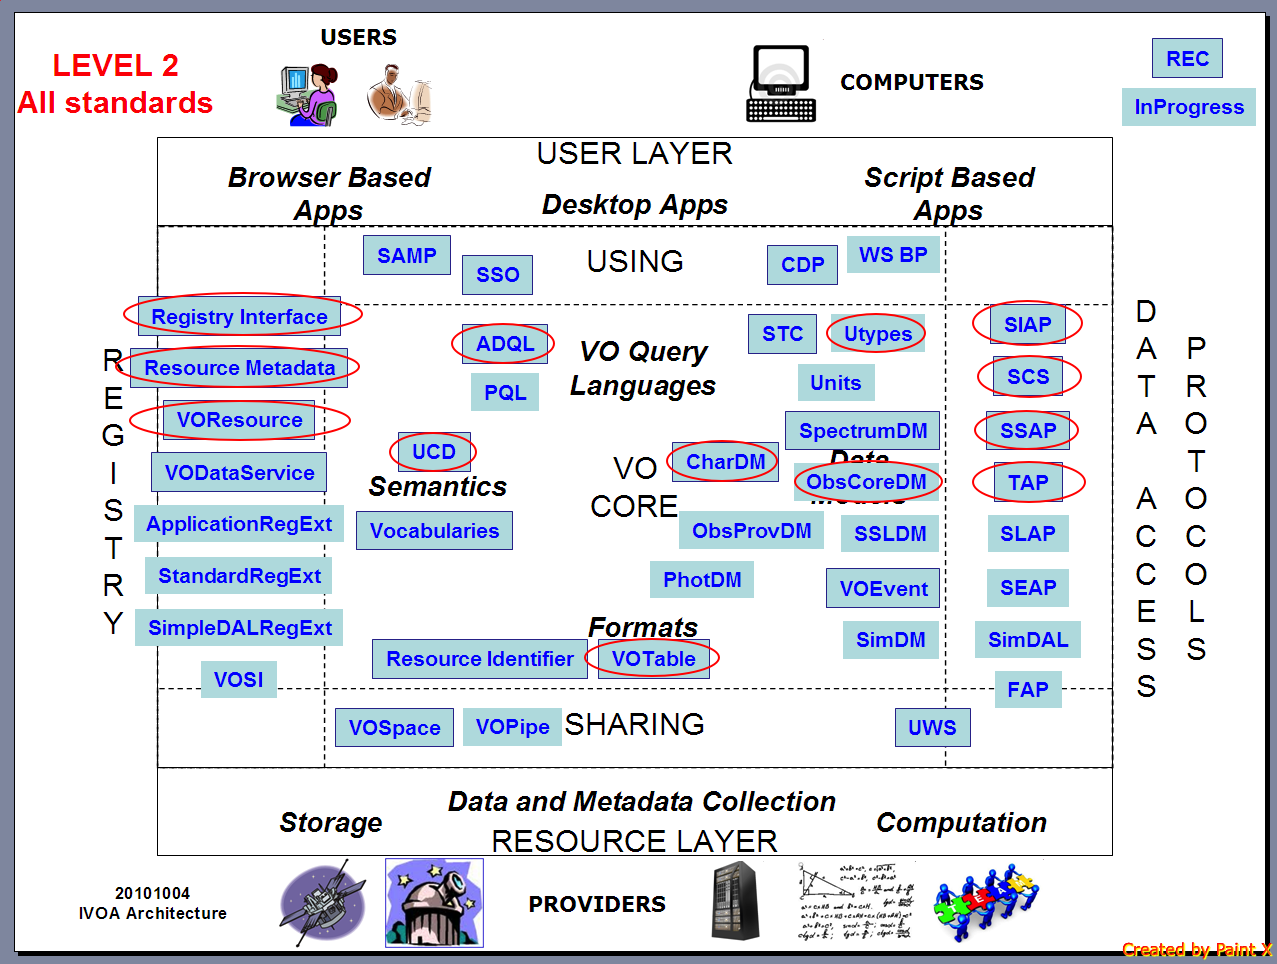
\includegraphics[width=0.45\textwidth]{images/arquitectura_2.png}
    \caption{Arquitectura de IVOA con los Protocolos y Estandares usados}
    \label{fig:ivoarch}
\end{figure}

\subsection{Arquitectura ChiVO}

Según las necesidades de lo radioastrónomos chilenos, los requerimientos y casos de
uso obtenidos a partir de ello y los modelos de datos compatibles con los estándares
de IVOA se ha creado una arquitectura y modelo de desarrollo.

\begin{figure}[h]
    \centering
    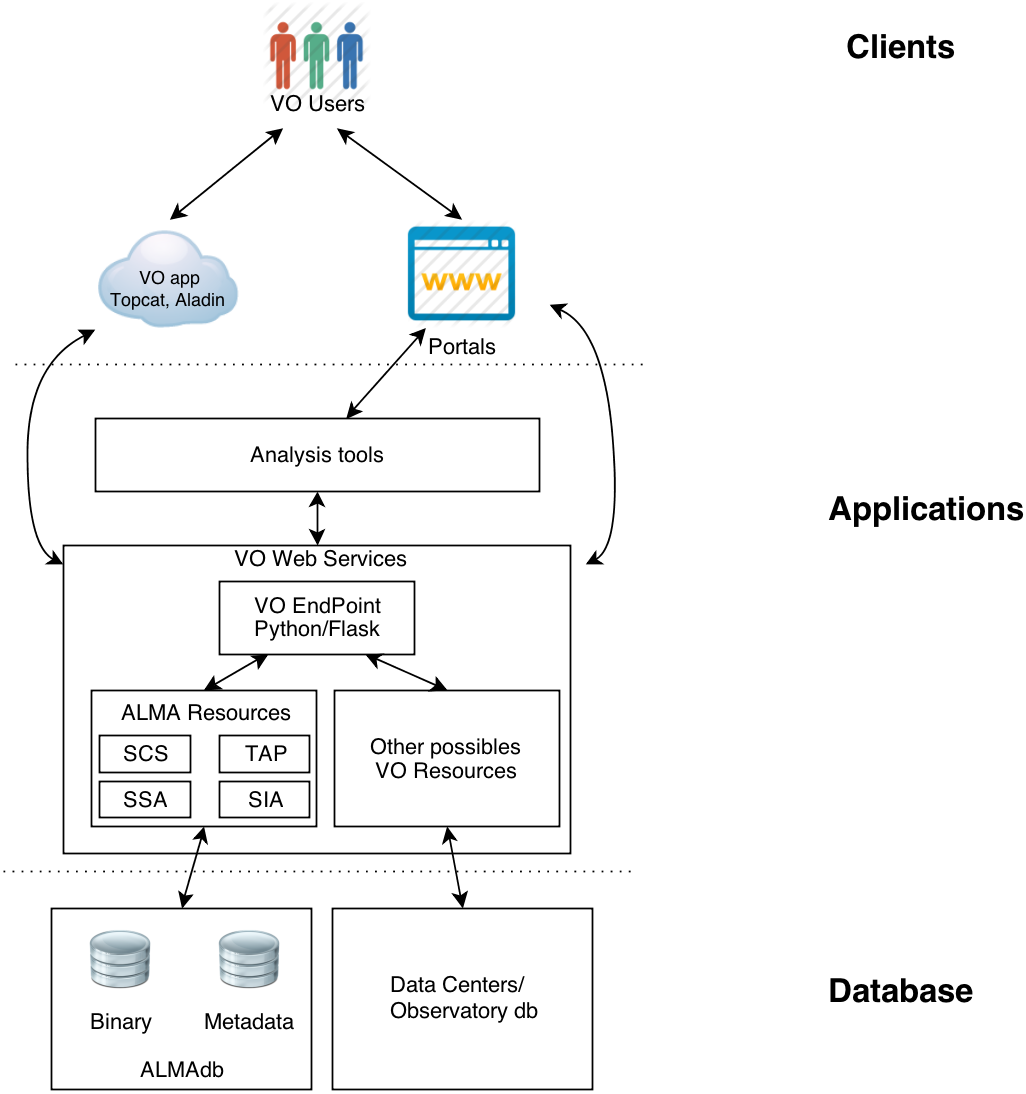
\includegraphics[width=0.45\textwidth]{images/chivo_capas.png}
    \caption{Arquitectura de ChiVO}
    \label{fig:chivoarch}
\end{figure}

\textbf{Capa de clientes}

Esta capa representa al usuario final y cómo facilita la comunicación entre el
usuario y los datos.
En esta capa el usuario realiza consultas a través de los protocolos de acceso
ofrecidos por ChiVO o a través de un formulario avanzado, utilizando aplicaciones
compatibles con VO y el portal web, respectivamente.
Una vez realizada la consulta, el sistema le retornará al usuario una lista que
describe objetos u observaciones encontrados (metadatos) y podrá acceder a ellos a
través de un enlace de descarga asociado a cada resultado.
Cabe destacar que gracias a la separación por capas, se logra flexibilidad y
escalabilidad en el sistema, para que independiente de una capa y otra, puedan
interactuar nuevas aplicaciones y portales con ChiVO, así como la adición de nuevas
fuentes de información a parte de ALMA.

Las consultas son recibidas por ChiVO a través de su endpoint de datos que recibe
consultas en HTTP, GET o POST, ante lo cual el endpoint retorna la lista de
resultados en una tabla en el formato XML (VOTable).
Para el caso del portal web, el VOTable es desplegado mostrado al usuario a través
de una herramienta web que permite la manipulación simple y eficiente de VOTables
llamada VOView.

\textbf{Capa de Aplicaciones}

En esta capa se encuentran los programas que procesan las consultas entre los
usuarios y los datos.
Cada estándar de IVOA requiere un mínimo de su propia implementación para ser
compatible con el VO, en el caso de estos protocolos de acceso sólo es necesaria la
recepción de consultas HTTP básicas junto a los parámetros de búsqueda requeridos.

La caja que representa a las herramientas de análisis es fundamental en la
eficiencia de ChiVO, esto es debido a que los datos a analizar por los astrónomos
suelen tener un gran tamaño y es costosa su transferencia, este problema se
resuelve acercando las herramientas de análisis y procesamiento al lugar donde están
almacenados los datos a procesar.

Dado que más adelante será necesario ofrecer búsquedas por otros datos que no sólo
provengan de ALMA, es necesaria cierta abstracción al momento de implementar esta
capa, ya que debe permitir a futuro interactuar con nuevos recursos pero siempre
manteniendo la compatibilidad de IVOA para que sea utilizable por aplicaciones
compatibles con el ecosistema de IVOA.

En esta capa también está en desarrollo un sistema capaz de resolver nombres
(tipo sesame pero para datos de ALMA) y el registro de ChiVO.

\textbf{Capa de Datos}

En esta capa se encuentran los recursos que tienen los datos y metadatos.
En esta parte se trabaja con una base de datos relacional para almacenar los
metadatos asociados al modelo de datos recomendado por IVOA Observation Core Data
Model, usando un framework desarrollado por el VO Alemán.
Esta es la parte que mas consume recursos, tanto en tiempo de computación (resuelve
las consultas hechas a las base de datos) y además almacena físicamente los datos.
Por efectos de prueba se está trabajando con un set de datos de 1TB, los cuales son
los archivos más reducidos del ciclo 0 de ALMA. Debido a esta limitancia se propone
el esquema de funcionamiento de la figura \ref{fig:dachs}, en donde pueden haber N 
servidores con DaCHS configurado apunando a M base de datos distribuidas o recplicadas.

\begin{figure}[h]
    \centering
    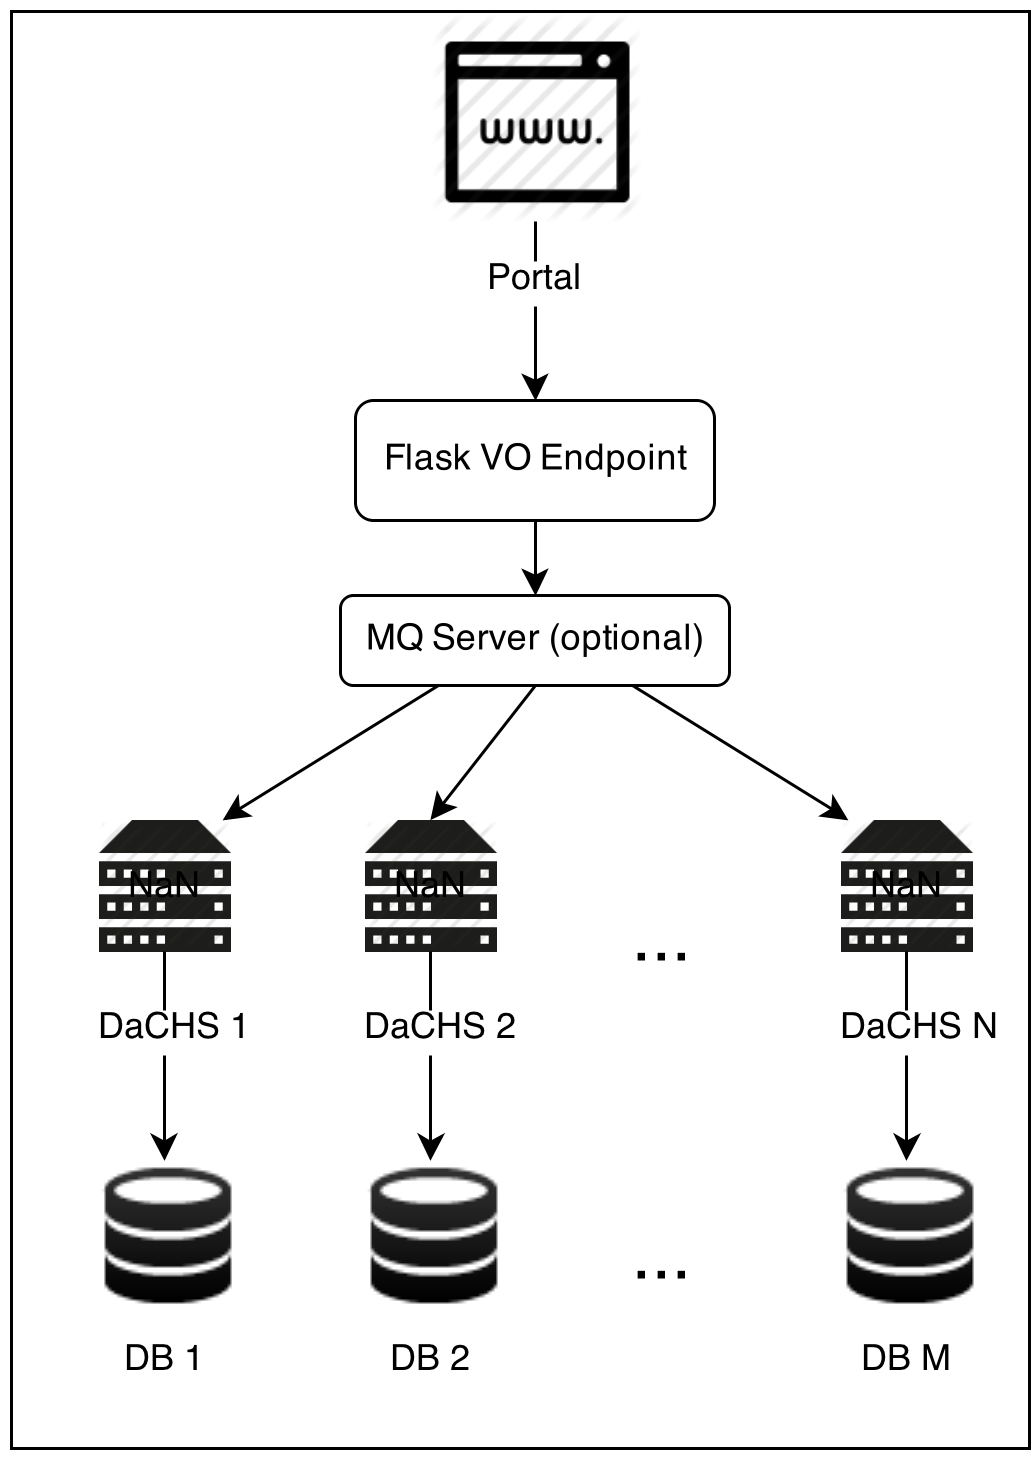
\includegraphics[width=0.45\textwidth]{images/interaccion.png}
    \caption{Configuración de distintas máquinas con base de datos replicadas o distribuidas}
    \label{fig:dachs}
\end{figure}

\subsection{Metadatos de los datos de ALMA}

Para poder construir la base de datos relacional con el modelo de datos ObsCore fue
necesario mapear campos desde el ALMA Science Data Model (ASDM) \cite{viallefond2009sdm}.

\begin{table}[h!t]
    \centering
    \caption{Campos del ObsCore y origen desde ASDM}
    \begin{tabular}{lr}
        \textbf{Campo ObsCore} & \textbf{ASDM} \\
        dataproduct\_type      & visibility \\
        calib\_level           & 1 \\
        obs\_collection        & ALMA \\
        obs\_id                & [ExecBlock.execBlockUID] \\
        obs\_publisher\_did    & [Cycle ID] \\
        access\_url            & [URL de ChiVO] \\
        access\_format         & application/x-asdm \\
        access\_estsize        & [main.dataSize] \\
        target\_name           & [Source.sourceName] \\
        s\_ra                  & [Source.direction] \\
        s\_dec                 & [Source.direction] \\
        s\_fov                 & [1.2 * lambda / Diametro antena] \\
        s\_region              & circle \\
        s\_resolution          & [1.2*lambda/(ExecBlock.baseRangeMax)] \\
        t\_min                 & [ExecBlock.startTime] \\
        t\_max                 & [ExecBlock.endTime] \\
        t\_exptime             & [main.interval] \\
        t\_resolution          & [mainTable.interval] \\
        em\_min                & [ExecBlock.baseRangeMin] \\
        em\_max                & [ExecBlock.baseRangeMax] \\
        em\_res\_power         & [spectralWindow.resolution] \\
        o\_ucd                 & em.mm \\
        pol\_states            & [Source.stokesParameter[numStokes]] \\
        facility\_name         & ALMA \\
        instrument\_name       & ALMA \\
    \end{tabular}    
    \label{table:obsasdm}
\end{table}

En la Tabla \ref{table:obsasdm} se muestra el resultado de la investigación, la primera
columna corresponde a las columnas de la clase Observation, la segunda columna
indica de donde se obtienen los datos para llenar la los campos de la primera
columna para el caso de los ASDM.

Para poder llenar los campos de la clase Observation es necesario escribir una
rutina capaz de operar sobre las tablas del ASDM (XML).
Actualmente existen múltiples herramientas en el Paquete de Aplicaciones de Software
Comunes de Astronomía (CASA, debido a sus siglas en inglés) \cite{petry2012analysing}.

\subsection{Tecnologías usadas}

Para el desarrollo de ChiVO se evaluaron distintas herramientas posibles de las
cuales se concluyó en cada capa:

\textbf{Endpoint}

Los framework que se evaluaron para la implementación del endpoint fueron:

\begin{description}
    \item[Ruby on Rails (RoR):] \hfill \\
        Es uno de los framework de desarrollo web más usados actualmente, su uso es
        mediante el concepto Modelo-Vista-Controlador (MVC).
        La razón por la cual no se eligió esta herramienta es porque era más grande
        de lo que se necesitaba.
    \item[Python/Flask:] \hfill \\
        Flask es un microframework diseñado especialmente para hacer webservices y
        herramientas web pequeñas.
        Lo que provee esta biblioteca es un marco de trabajo para la creación de
        aplicaciones web que puedan ser accedidas mediante distintos métodos HTTP.
        Existe mucha documentación y comunidad activa que permite implementar y
        solucionar problemas de forma rápida.
\end{description}

\textbf{ALMA Resource}

Dentro de los toolkits de DAL recomendados por IVOA, se testearon los siguientes:

\begin{description}
    \item[SAADA:] \hfill \\
        Desarrollado por el VO Francés, es una herramienta bastante útil del punto
        de vista usuario, posee excelente documentación y manual de instalación,
        incluso la instalación se mediante GUI.
        Está desarrollado en Java y su correspondiente despliegue se hace usando
        Tomcat.
        Por lo que se pudo apreciar desde la página web no es OpenSource.
        Es posible configurar servicios SCS/SIA/SSA/TAP.

    \item[VO-Dance:] \hfill \\
        Desarrollado por el VO Italiano, es una herramienta en Java en su Backend,
        y Python en su Frontend (Framework Django).
        Lo destacable de esta herramienta es que trabaja usando MySQL como motor de
        base de datos principal, y según lo conversado con los desarrolladores están
        probando PostgreSQL actualmente.
        La herramienta no es OpenSource y la documentación de instalación y
        configuración es básica, ya que aún continúa en desarrollo. SCS/SIA/SSA/TAP.

    \item[openCADC:] \hfill \\
        Desarrollado por el VO Canadiense, es una herramienta OpenSource escrita en
        Java, utilizada actualmente en el ALMA Science Archive.
        Este toolkit es uno de los más robustos, contiene distintos paquetes con
        servicios a ser utilizados en el webservice, sin embargo no existe
        documentación de instalación y configuración, y para poder probarlo fue
        necesario contactar directamente al desarrollador principal.
        Es posible configurar servicios TAP.

    \item[DaCHS:] \hfill \\
        Desarrollado por el VO Alemán, es una herramienta OpenSource escrita en
        Python.
        Es uno de los toolkits DAL más usados por los VO, ya que posee una amplia
        documentación de instalación y configuración.
        Es posible configurar servicios SCS/SIA/SSA/TAP.
\end{description}

%\vspace{0.5cm}
\begin{table*}[h!t]
\centering
\caption{Resumen de los toolkits en tabla comparativa}
\begin{tabular}{lrrrrr}
    {\bf Toolkits} & {\bf Lenguaje} & {\bf OpenSource} & {\bf Documentación} & {\bf Servicios} & {\bf Último update}  \\
    SAADA          & Java           & No               & Si                  & SCS/SIA/SSA/TAP & Mayo 2012     \\
    VO-Dance       & Java/Python    & No               & No                  & SCS/SIA/SSA/TAP & Dicimbre 2012 \\
    openCADC       & Java           & Si               & No                  & TAP             & ---           \\
    DaCHS          & Python         & Si               & Si                  & SCS/SIA/SSA/TAP & Junio 2013    \\
\end{tabular}
\label{table:toolkits}
\end{table*}

\textbf{Interfaz Usuario}

Inicialmente la interfaz usuario o frontend iba a contener solo vistas, por lo que
el desarrollo podía ser en prácticamente cualquier lenguaje o framework, como por
ejemplo HTML, PHP, Django o RoR. Sin embargo con los requerimientos de la
plataforma, especialmente el de capa de usuarios, se decidió inclinarse por un
framework MVC que fuese lo suficientemente ágil y compatible con el resto de
servicios, por lo que se eligió RoR. En la cual se usa principalmente HTML y
Javascript.

\section{Estado de avance}

Para comenzar el desarrollo de ChiVO fue necesario identificar aparte de los
requerimientos y casos de uso, las interacciones que los usuarios realizarán
con el sistema. El diagrama de secuencia de interacción entre el usuario y
ChiVO se puede ver en la figura \ref{fig:secuencia}.
En base a este diagrama, requerimientos y tecnologías utilizadas el estado de
avance se especificará por cada capa de abstracción.

\begin{figure*}[h!t]
    \centering
    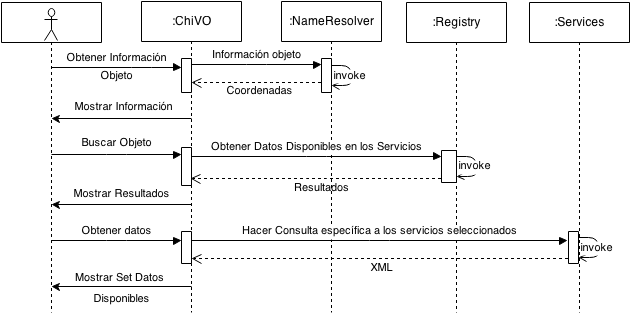
\includegraphics[width=0.7\textwidth]{images/secuencia.png}
    \caption{Diagrama de secuencia entre Usuario y ChiVO}
    \label{fig:secuencia}
\end{figure*}

\subsection{Frontend}

Dento del diagrama de secuencia, el Frontend es el VO-Client, es decir, está a cargo
de generar la interacción entre los usuarios y los demás elementos dentro del
sistema.

Actualmente se generó un frontend en RoR que permite interactuar con:

\begin{description}
    \item[Resolver nombres]:\hfill \\
        a partir de un nombre (String) retorna la posición de un objeto en
        coordenadas celestiales usando el servicio SESAME de Astrogrid.
    \item[Registro]: \hfill \\
        busca servicios dentro del endpoint, y luego según lo que necesite el
        usuario elige sobre cuales trabajar para hacer consultas.
    \item[Servicios]: \hfill \\
        consulta a diferentes servicios web que proveen datos mediante cierto
        protocolo y unifica los resultados en un XML VOTable para ser desplegados
        en forma ordenada usando una biblioteca de javascript VOView.
\end{description}

\subsection{Endpoint}

El Endpoint está a cargo de generar una interacción transparente entre los clientes
de VO y los posibles recursos que se configuren.
En este caso el Endpoint genera una interfaz para los servicios configurados por el
Backend y los disponibles a través del registro de VO-Paris.
VO-Paris posee una Web API en REST que permite consultar por recursos y retorna un
archivo JSON con resultados.

\subsection{Backend}

Actualmente ALMA le facilita a ChiVO datos públicos, los cuales incluyen ASDM,
Measurement \cite{petry2012analysing}, FITS \cite{wells1981fits}, de los cuales es
necesario extraer los metadatos del ObsCoreDM para ser ingresados a la base de datos.

\begin{figure}[h!t]
    \centering
    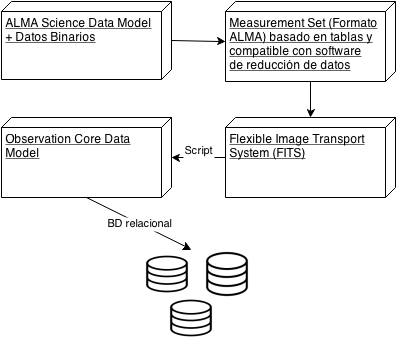
\includegraphics[width=0.45\textwidth]{images/metadata.png}
    \caption{Proceso transformación desde Frontend de ALMA hasta la base de datos
             de ChiVO}
    \label{fig:metadata}
\end{figure}

El procedimiento se hace a través de un programa, el cual usando el framework de
backend DaCHS \cite{dachs}, permite configurar recursos y servicios mediante
archivos de configuración Resource Descriptor \cite{dachsorguide}.
Una vez creadas las entradas en la base de datos y configurados los servicios SCS,
SSAP, SIAP, TAP se pueden acceder mediante las consultas definidas en cada
protocolo.



\section*{Agradecimientos}
Los autores quieren expresar su agradecimiento al Fondo de Fomento al
Desarrollo Científico y Tecnológico (FONDEF), quienes hacen posible este
trabajo.

\section{Referencias}
\bibliographystyle{plain}
\bibliography{ccs}

\end{document}
